
\chapter{Conception}
\vspace{3cm}
\minitoc
\clearpage

\label{Chapitre3}


\section{Introduction}

\begin{onehalfspace}

\lettrine[nindent=1em,lines=3]{D}ans les chapitres précédents, nous avons exploré quelques techniques qui ont été proposées dans la littérature et qui ont un impact sur la consommation d'énergie.\medskip

Notre objectif principal est de proposer et d'implémenter une nouvelle stratégie de migration des machines virtuelles, Et cela dans le but d'améliorer certaines métriques de performance telle que la consommation d'énergie sans dégrader les contraintes du contrat SLA.\medskip

Le présent chapitre permet d'expliquer notre démarche en décrivant ses différentes phases, les algorithmes nécessaires pour son fonctionnement ainsi que les différentes étapes formalisées à l'aide du langage UML.
\end{onehalfspace}

\section{Approche proposée}
\begin{onehalfspace}
L’objectif de ce travail étant de proposer une stratégie basée sur la migration des machines virtuelles. Cette proposition permet de sélectionner le nombre minimum des machines virtuelles nécessaire à faire migrer à partir d’une machine physique.
L’avantage de cette stratégie est qu’elle permet d’augmenter considérablement le taux d’utilisation et de réduire la demande en énergie. L’idée de base est de concentrer les traitements de données sur une machine physique et d’éteindre les autres.

\end{onehalfspace}

\section{Architecture du système}
\begin{onehalfspace}
Dans cette partie, nous allons décrire le fonctionnement de notre modèle tout en formalisant et en utilisant une architecture qui sera la base de notre approche. Comme c’est illustrée dans la figure \ref{Architecture du système}, cette architecture est décrite par l’ensemble des composants suivants :
\clearpage
\begin{figure}[!h]
\begin{center}
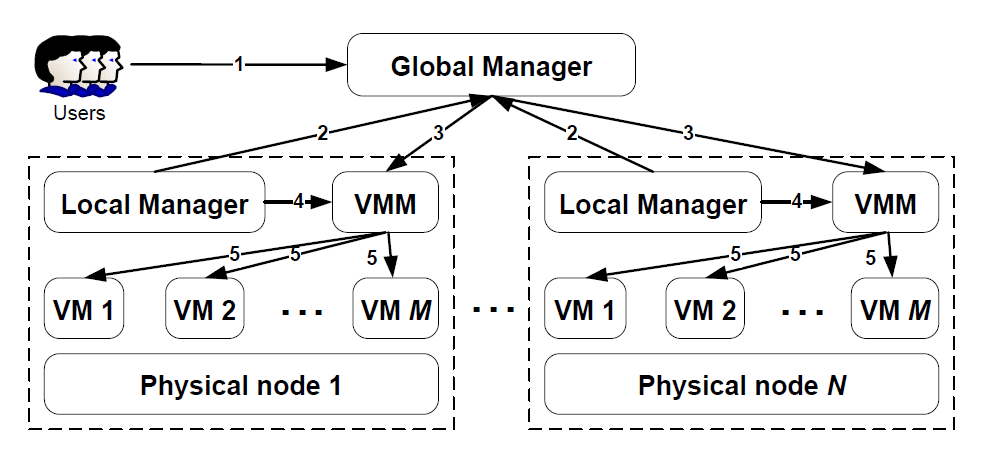
\includegraphics[scale=0.43]{figures/4.png} 
\end{center}
\caption{Architecture du système}
\label{Architecture du système}
\end{figure}
\begin{enumerate} [label=\Roman*)]
%\item \textbf{Data Center :} Un data center est une entité informatique composée d’un ensemble de machines physiques. Il est caractérisé par le nombre et la vitesse des processeurs, la capacité de la mémoire et de stockage, la bande passante ainsi que le coût de chaque ressource.
%\item \textbf{ Broker :} Le Broker assure la gestion des VMs dans plusieurs data centers et le routage du trafic vers les data centers appropriés. Il choisit aussi le data center qui fournit le meilleur  service pour les demandes envoyées par chaque utilisateur. Le Broker est responsable de la communication entre les utilisateurs et les data centers..
\item \textbf{Physical node :} Une machine physique est caractérisée par le nombre des VMs, la capacité, le nombre des requêtes arrivées, la vitesse du CPU et nombre de cores.
\item \textbf{VMs :}  Une machine virtuelle consiste à créer plusieurs environnements d'exécution sur une seule machine physique. Elle fournit à chaque utilisateur un service selon la demande.
\item \textbf{VM Manager (VMM):} Assure le suivi de la disponibilité des machines virtuelles et de leur utilisation des ressources. Il est chargé du provisionnement des nouvelles machines virtuelles ainsi que la réaffectation des VMs d’une machine physique à une autre afin d’adapter le placement.
\item \textbf{Local managers :} Les gestionnaires locaux se trouvent sur chaque noeud comme un module du VMM. Leur objectif est le suivi continu d’utilisation du processeur d’un noeud, le redimensionnement de la VM en fonction de leurs besoins en ressources et la prise de décision (quand et où les machines virtuelles doivent être migrées à partir d'un noeud physique).

\item \textbf{Global manager :} Il réside sur un nœud maître et recueille des informations auprès des gestionnaires locaux pour maintenir la vue globale de l'utilisation des ressources.
\end{enumerate}

Les gestionnaires locaux se trouvent sur chaque nœud en tant que module du moniteur de machine virtuelle (VMM). Leur objectif est le suivi continu d'utilisation du processeur d'un nœud, le redimensionnement de la VM en fonction de leurs besoins en ressources et la prise de décision (quand et où les machines virtuelles doivent être migrées à partir du nœud d'accueil) (4). Ils permettent aussi  de recevoir des requêtes à partir des clients (1). Le gestionnaire global réside sur un nœud maître et recueille des informations provenant des responsables locaux pour maintenir la vue d'ensemble de l'utilisation des ressources (2). Le gestionnaire global émet des commandes pour l'optimisation du placement VM (3). VMM effectue des redimensionnements réels et la migration des machines virtuelles ainsi que des changements dans les états d'alimentation des nœuds (5).
\end{onehalfspace}

\subsection{Calcul de la consommation d'énergie}
\begin{onehalfspace}

Ils existent plusieurs méthodes pour calculer la consommation d'énergie, parmi lesquels
nous avons utilisé la "méthode puissance par rapport à l'utilisation" : De nombreuses études, \cite{ref34}, \cite{ref35} ont montré que la consommation d'énergie par les serveurs peut être décrite par une relation linéaire entre la consommation d'énergie et l'utilisation du processeur. Ces études confirment qu'une puissance moyenne consommée par un serveur inactif est de 70\% de l'énergie consommée par rapport à un serveur pleinement utilisé et d'après \cite{ref36} , si l'utilisation du processeur est supérieure à 30\%, la valeur inférieure est toujours 0,3. Donc, ils ont défini la consommation d'énergie $P(u)$ par la Formule \ref{form1} :\bigskip

\begin{equation}
P(u) = Pmax \ast (0.7 + 0.3u)
\label{form1}
\end{equation}
\bigskip

\textbf{Tel que :}
$Pmax$ = 250w pour des serveurs modernes. La constante 0.7 est la puissance moyenne consommée par un serveur inactif quand le serveur est pleinement utilisé. \textit{u} : est l'utilisation du processeur. Comme l'utilisation de CPU peut changer avec le temps en raison de la variabilité de la charge de travail, il s'agit d'une fonction du temps: \textit{u(t)}. Par conséquent, pour définir la consommation d'énergie totale par un serveur, nous utilisons l'équation \ref{form3} \bigskip .\bigskip
\begin{equation}
E_{S} = \int_{t} {P(u(t)) dt}
\label{form3}
\end{equation}
\bigskip

Donc la consommation d'énergie par rapport à un data center est calculée par la Formule \ref{form2} \cite{ref37} : \bigskip

\begin{equation}
E_{D} = \frac{\sum_{j=1}^{m} P(u)_j}{m}
\label{form2}
\end{equation}
\bigskip

\textit{m} : nombre de machines physiques dans un data center.
\end{onehalfspace}
\subsection{Coût de la migration à Chaude des VMs}
\begin{onehalfspace}
La migration à chaude a un impact négatif sur les performances des applications en cours d'exécution dans une machine virtuelle pendant une migration. Voorsluys et al  \cite{ref38}, ont effectué une étude expérimentale pour étudier la valeur de cet impact et trouver un moyen de modélisation. Ils ont découvert que la dégradation des performances et des temps d'arrêt dépendent du comportement de l'application, c'est à dire, combien de pages mémoires sont mise à jour par l'application pendant son exécution. Pour les applications de web,  la dégradation de performance moyenne et  le temps d'arrêt peut être estimé à 10\% de l'utilisation du processeur. Cela signifie que chaque migration peut entraîner une certaine violation SLA. Il est donc essentiel de réduire au minimum le nombre de migrations de machines virtuelles. La durée d'une migration à chaude dépend de la quantité totale de mémoire utilisée par la machine virtuelle et la bande passante disponible. Pour nos expériences, nous définissons la dégradation des performances expérimentées par les $VM_j$ par la formule \ref{form4} \cite{ref43}: \bigskip

\begin{align}
 T_{m_{j}} = \frac{M_{j}}{B_{j}} \\
 U_{d_{j}} = 0.1\cdot \int_{t_{0}}^{t_{0}+T_{m_{j}}} {u_{j}(t) dt} \label{form4}
\end{align}
\bigskip

Où $U_{d_{j}}$ est la dégradation totale de performance par la $VM_j$, $t_{0}$ le temps où la migration commence, $T_{m_{j}}$ est le temps nécessaire pour terminer la migration, $u_{j}(t)$ est l'utilisation de la CPU par la $VM_j$, $M_{j}$ est la quantité de mémoire utilisée par la $VM_j$ et $B_{j}$ est la bande passante réseau disponible.
\end{onehalfspace}

\subsection{Violation de SLA}
\begin{onehalfspace}
Les exigences de la qualité de service sont extrêmement importantes pour le Cloud computing. Elles sont généralement formalisées sous forme de SLA\footnote{Service Level Agreement (SLA) est un document qui définit la qualité de service requise entre un prestataire et un client.}. Le contrat SLA peut être déterminé en termes de plusieurs contraintes  telles que le débit minimum ou le  temps de réponse maximum fourni par le système déployé. Etant donné que ces caractéristiques peuvent varier selon les applications, il est nécessaire de définir une métrique générique qui peut être utilisée dans notre simulation pour estimer le niveau du SLA qui est délivré par l’infrastructure. Pour ce qui nos concerne, nous définissons le niveau global de violation SLA causé par le système  comme une fraction de la différence entre les MIPS\footnote{MIPS : \textit{Million d'instructions par seconde}, unité de mesure des processeurs.} demandées par toutes les machines virtuelles $U_{r_{j}} (t)$ et les MIPS réellement alloués $U_{a_{j}} (t)$ . Cela est relatif au total des MIPS demandés au cours de la durée de vie des machines virtuelles ( voir équation \ref{form5}) \cite{ref43} . Où $M$ est le nombre de machines virtuelles.\medskip
\begin{align}
SLA = \dfrac{\sum_{j=1}^{M} \int_{t} U_{r_{j}} (t) - U_{a_{j}} (t) dt}{\sum_{j=1}^{M} \int_{t} U_{r_{j}} (t)}
\label{form5}
\end{align}\medskip

Cette métrique représente le pourcentage de la performance du CPU qui n'est pas afféctée lorsqu'elle est demandée par les applications relatives à la demande totale.
\end{onehalfspace}
\section{La stratégie de la minimisation des migrations des machines virtuelles}
\begin{onehalfspace}
Notre approche est divisée en deux phases: la sélection des VM à faire migrer  et l'allocation des VMs (voir Figure \ref{DiAMM}).

\begin{enumerate}
\item \textbf{Phase 1 : }Nous sélectionnons dans cette phase les machines virtuelles qui doivent être migrées (quelle VM doit-on choisir pour  faire une migration?) ;
\item \textbf{Phase 2 : }Les machines virtuelles choisies sont placées dans  les machines physiques à l’aide d’un algorithme de placement (quel  est le nouvel emplacement de la VM?).
\end{enumerate} 
\end{onehalfspace}
\clearpage
\begin{figure}[!h]
\begin{center}
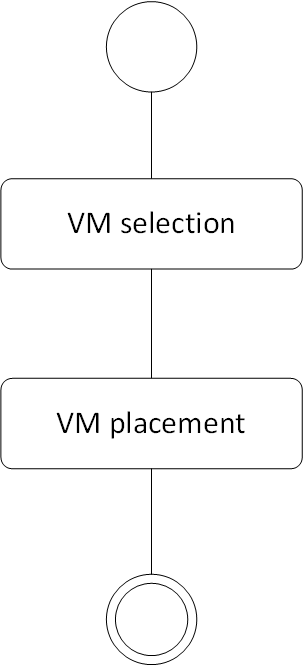
\includegraphics[scale=0.5]{figures/6.png} 
\end{center}
\caption{Diagramme d'activité de la migration des machines virtuelles}
\label{DiAMM}
\end{figure}



\subsection{Sélection des machines virtuelles}
\begin{onehalfspace}
Pour déterminer quand les machines virtuelles doivent être migrées, nous utilisons deux seuils d'utilisation du CPU (voir Figure \ref{DiASe}).
\subsubsection{Seuils d'utilisation fixe}
L’idée est de fixer deux seuils d’utilisation de CPU (seuil supérieur et seuil inférieur) et de garder l’utilisation totale du CPU de toutes les machines physique entre ces seuils. Si l’utilisation du CPU d’une machine physique est en dessous du seuil inférieur, toutes les VMs doivent être migrées de cette PM. Cette dernière est mise après en état hors tension (éteinte).

Si l’utilisation du CPU de la machine physique dépasse le seuil supérieur, on cherche la meilleure machine virtuelle pour faire une migration, afin de réduire l’utilisation de CPU. La meilleure VM est celle qui répond à deux conditions !
\begin{enumerate} [label=\Roman*)]
\item la machine virtuelle doit avoir une utilisation plus grande que la différence entre l’utilisation globale de CPU et le seuil supérieur.
\item la différence entre le seuil supérieur et la nouvelle utilisation de CPU est la plus petite. Si une telle VM n’existe pas, l’algorithme sélectionne la VM avec la plus grande utilisation CPU.
\end{enumerate}


\subsubsection{Seuils d'utilisation dynamique}
Comme mentionné précédemment, les seuils fixes ne sont pas adaptés pour un environnement avec des charges de travail dynamiques et imprévisibles. Cet environnement possède différents types d'applications qui peuvent partager la même ressource physique. Le système doit être capable d'ajuster automatiquement son comportement en fonction des modèles de charge de travail exposées par les applications. C'est pourquoi, nous utilisons une nouvelle technique pour calculer automatiquement les deux seuils d'utilisation CPU. Cette technique est basée sur sur une analyse statistique des données historiques recueillies au cours de la durée de vie des machines virtuelles \cite{ref44}. Nous allons présenter maintenant les formules permettant de calculer les seuils fixes.

\begin{enumerate}
\item \textbf{Seuil supérieur $T_{U_{i}}$:}
Nous avons calculé seuil supérieur $T_{U_{i}}$ comme montré dans \ref{tI}.
\begin{center}
\begin{equation}
U_{i} = \sum_{j=1}^{m} u_{j}
\end{equation}
\begin{equation}
S_{U_{i}} = \sqrt{\sum_{j=0}^{m} u_{j}^{2}}
\end{equation}
\begin{equation}
T_{U_{i}} = 1 - (((P_{uu} \ast S_{U_{i}}) + U_{i}) - ((P_{ul} \ast  S_{U_{i}}) + U_{i})
\label{tI}
\end{equation}
\end{center}
$u_{j}$ : L'utilisation du CPU de la machine virtuelle \textit{j}.\\
$m$ : Le nombre de machines virtuelles.\\
$U_{i}$ : L'utilisation du CPU de la machine physique \textit{i}.\\
$P_{uu}$ : égale à 95\% \cite{ref44}.\\
$P_{ul}$ : égale à 90\% \cite{ref44}.
\item \textbf{Seuil inférieur $T_{l}$:}
Nous avons calculé seuil inférieur $T_{l}$ comme montré dans 3.12.
\begin{center}
\begin{equation}
U_{i} = \frac{1}{m}\sum_{j=1}^{m} u_{j}
\end{equation}
\begin{equation}
S_{U_{i}} = \sqrt{(\sum_{j=0}^{m} u_{j} - U_{i})^{2}}
\end{equation}

\[
\label{TL}
T_{l} = \left\{
\begin{array}{r c l l l r}
U_{i} - (P_{l}*S_{U_{i}}) &,\textbf{Si}& L'utilisation& du& CPU < 0.3& (3.12)\\
0.3 &,\textbf{Si}& L'utilisation& du& CPU > 0.3
\end{array}
\right.
\]
\end{center}
$u_{j}$ : L'utilisation du CPU de la machine virtuelle \textit{j}.\\
$m$ : Le nombre de machines virtuelles.\\
$U_{i}$ : L'utilisation du CPU de la machine physique \textit{i}.\\
$P_{l}$ : égale à 90\% \cite{ref44}.
\end{enumerate}

\subsubsection{Phase de sélection des VMs}

La Figure \ref{DiASe} montre un diagramme d’activité qui résume la phase de sélection des machines virtuelles:
\clearpage
\begin{figure}[!h]
\begin{center}
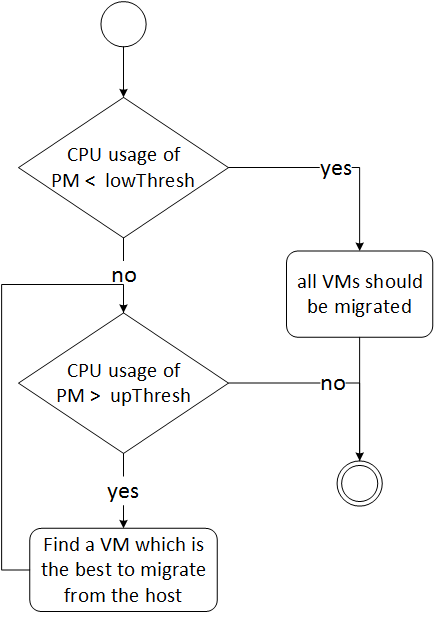
\includegraphics[scale=0.5]{figures/7.png} 
\end{center}
\caption{Diagramme d'activité de sélection des machines virtuelles}
\label{DiASe}
\end{figure}
L'algorithme \ref{ASe} illustre le pseudo-code de la procédure de sélection des machines virtuelles.
\clearpage
\RestyleAlgo{ruled}

\begin{algorithm}[!h]
%\DontPrintSemicolon
\SetAlgoVlined

\LinesNumbered
\Entree{hostList, vmList} \Sortie{migrationList}
\BlankLine
vmList.sortDecreasingUtilization()\;
\PourCh{h \textbf{dans} hostList}
{
	hUtil $\leftarrow$ h.util()\;
	bestFitUtil $\leftarrow$ MAX\;
	\Tq {hUtil $>$ h.upThresh()}
	{
		\PourCh{vm \textbf{dans} vmList}
		{
			\eSi{vm.util() > hUtil - h.upThresh()}
			{
				t $\leftarrow$ vm.util() - hUtil + h.upThresh()\;
				\uSi{t < bestFitUtil}
				{
					bestFitUtil $\leftarrow$ t\;
					bestFitVm $\leftarrow$ vm\;
				}
			}{
				\uSi{bestFitUtil = MAX}
				{
					bestFitVm $\leftarrow$ vm\;
				}\textbf{break}\;
			}
		}
		hUtil $\leftarrow$ hUtil - bestFitVm.util()\;
		migrationList.add(bestFitVm)\;
		vmList.remove(vm)\;
	}
	\Si{hUtil < h.lowThresh()}
	{
		migrationList.add(h.getVmList())\;
		vmList.remove(h.getVmList())\;
	}
}
\Retour{migrationList}\;
\caption{Algorithme de la sélection des machines virtuelles}
\label{ASe}
\end{algorithm}
L’algorithme \ref{ASe} est composé de deux parties :
La première partie de la ligne 5 jusqu’à la ligne 18 s’agit d’une boucle qui permet de réduire l'utilisation totale du CPU en dessous de seuil supérieur par sélection de quelques VMs à faire migrer. 
La seconde partie de la ligne 19 jusqu’à la ligne 21, il permet de vérifier si le seuil inférieur est violé, alors toutes les machines virtuelles seront migrées.   
\end{onehalfspace}
\subsection{Placement des machines virtuelles MBFD}
\begin{onehalfspace}
Pour déterminer l’emplacement des VMs migrées, nous utilisons l’algorithme MBFD\footnote{Modified Best Fit Decreasing (MBFD)}. Cet algorithme tri les  machines virtuelles dans l’ordre décroissant de leur utilisation de CPU. Il alloue  par la suite chaque VM dans une PM qui offre une consommation d’énergie minimale grâce à cette allocation (voir Figure \ref{DiAPl}).

La Figure \ref{DiAPl} montre un diagramme d’activité qui résume la phase de placement des machines virtuelles:

\begin{figure}[!h]
\begin{center}
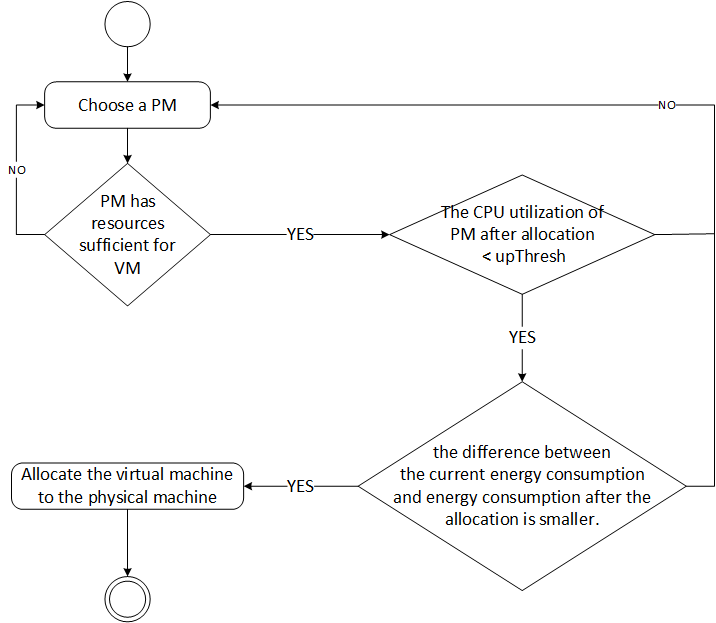
\includegraphics[scale=0.5]{figures/8.png} 
\end{center}
\caption{Diagramme d'activité de placement des machines virtuelles (MBFD)}
\label{DiAPl}
\end{figure}
\medskip
L'algorithme \ref{MBFD} illustre le pseudo-code de la procédure  de placement des machines virtuelles. 
\clearpage
\RestyleAlgo{ruled}

\begin{algorithm}[!h]
%\DontPrintSemicolon
\SetAlgoVlined

\LinesNumbered
\Entree{hostList, vmList} \Sortie{allocation of VMs}
\BlankLine
vmList.sortDecreasingUtilization()\;
\PourCh{vm \textbf{dans} vmList}
{
	minPower $\leftarrow$ MAX\;
	allocatedHost $\leftarrow$ NULL\;
	\PourCh{host \textbf{dans} hostList}
	{
		\Si{host a suffisamment de ressources pour vm}
		{
			power $\leftarrow$ estimatePower(host, vm)\;
			\Si{power < minPower}
			{
				allocatedHost $\leftarrow$ host\;
				minPower $\leftarrow$ power\;
			}	
		}
	}
	\Si{allocatedHost $\neq$ NULL}
	{
		allouer vm à allocatedHost\;
	}
}
\Retour{allocation}\;
\caption{Algorithme de placement des machines virtuelles (MBFD)}
\label{MBFD}
\end{algorithm}
L’algorithme \ref{MBFD} est composé de deux boucles imbriquées, la première boucle (ligne 2) permet de parcourir la liste des VMs à faire migrer. La seconde boucle (ligne 5) permet de parcourir la liste de toutes les PMs pour placer les VMs.

La complexité de l'algorithme \ref{MBFD} (MBFD) est $n*m$ , où \textit{n} est le nombre de noeuds et \textit{m} est le nombre des machines virtuelles qui doivent être migrées.
\end{onehalfspace}
\clearpage
\section{Conclusion}
\begin{onehalfspace}
Dans ce chapitre, nous avons présenté et décri les différentes étapes de notre stratégie proposée afin de minimiser le nombre de migration des machines virtuelles et par conséquence nous réduisant la consommation d’énergie .\medskip

Nous avons décrit le fonctionnement de notre proposition à l’aide d’un ensemble d'algorithmes, de formules et de diagrammes pour faciliter l'étude et la compréhension de notre proposition, d'une part, et pour donner un schéma général du travail demandé d'autre part.\medskip

En vue de concrétiser cette stratégie, nous allons décrire son implémentation dans le prochain chapitre sous le simulateur CloudSim, cela en utilisant le langage de programmation Java et l'environnement Netbeans.\medskip
\end{onehalfspace}
